\section{Sequential algorithm for Multilinear Detection} 
\label{sec:seq}
We briefly discuss the algorithm of Koutis \cite{koutis:icalp08}, which forms the basis of our paper. An important property is that for any $v_i \in \mathbb{Z}_2^k$, the square of the term $(v_0 + v_i) \in \mathbb{Z}_2[\mathbb{Z}_2^k]$ evaluates to 0:
{\small
$$
(v_0 + v_i)^2 = v_0^2 + 2(v_0\cdot v_i) + v_i^2 = v_0 + (0\mod 2)v_i + v_0 = 2v_0 = 0.
$$}

The main idea in the algorithm of \cite{koutis:icalp08} is that, if we evaluate a polynomial 
over the ``right" algebra, monomials that have square terms evaluate to 0, and the remaining terms,
which are multilinear, do not cancel out, with some probability.
Then, a polynomial $P(X)$ has a $k$ multilinear term if $P(X) \neq 0$. 

We can show that, if we choose a $v_i \in \mathbb{Z}_2^k$ uniformly at random and set $x_i = v_0 + v_i$, then a multilinear monomial does \textbf{not} evaluate to $\bar 0$ with high probability, whereas a monomial with squares is always $\bar 0$ (as in the box above).
The algorithm was later refined in \cite{williams2009finding} by evaluating the polynomial over the group algebra $GF(2^{3 + \log_2k})[\mathbb{Z}_2^k]$, where $GF(p)$ is the finite field of order $p$ \cite{mullen2007finite}. A polynomial $P(x_1,\ldots,x_n)$ with variables from $GF(2^{3 + \log_2k})[\mathbb{Z}_2^k]$ can be evaluated in time $O(2^k poly(n))$ and space $O(kpoly(n))$, resulting in Theorem \ref{theorem:kmld}.

\begin{theorem}[Koutis \cite{koutis:icalp08} and Williams \cite{williams2009finding}]
\label{theorem:kmld}
There exists an algorithm that, given an instance $P(x_1,\ldots,x_n)$ of the \textsc{$k$-MLD} problem, correctly returns ``no" if $P(X)$ does not contain a $k$ multilinear term. Otherwise, if $P(X)$ has a $k$ multilinear term, it returns ``yes" with probability at least 1/5. 
The algorithm has time complexity $O(2^k poly(n))$ and space complexity $O(2^k poly(n))$.
\end{theorem}

At a high level, the algorithm of \cite{koutis:icalp08} involves the following steps.
\begin{enumerate}
\item For each variable $x_i$, sample a vector $v_i$ uniformly at random from $\mathbb{Z}_2^k$ and assign $x_i = (v_0 + v_i) \in \mathbb{Z}_2[\mathbb{Z}_2^k]$.
\item Evaluate the polynomial $P(x_1,\ldots,x_n)$ on this random assignment.
\item If $P(x_1,\ldots,x_n) \neq \bar{0}$ return ``yes"; otherwise, return ``no",
where $\bar{0}$ is the additive identity of the group algebra.
\end{enumerate}

%For the case when a multilinear monomial appears an odd number of times in $P(X)$, Koutis proposed a randomized algorithm that runs in $O(2^k poly(n))$ time and returns an affirmative answer with probability at least $1/4$ \cite{koutis:icalp08}. This algorithm was later extended by Williams \cite{williams2009finding} to allow even repetitions.

%It has been shown that many parameterized graph problems reduce to \textsc{$k$-MLD} \cite{koutis:icalp08,williams2009finding,guillemot2013finding,koutis2012constrained} by efficiently encoding subgraphs of interests as monomials. For example, in the $k$-path problem\footnote{In the $k$-path problem, we are given an unweighted graph $G(V,E)$, and the goal is to decide whether or not there is a simple path containing exactly $k$ nodes in $G$.}, it is possible to recursively construct a polynomial in which each term represents a walk of length $k$, and only multilinear terms correspond to simple paths. Our algorithms in Section \ref{sec:proposed} are based on this methodology: we encode subgraphs of a given size and weight as polynomials, and only connected subgraphs of size at most $k$ where all the nodes are different are multilinear terms.



%Now, we define a group algebra $\mathbb{Z}_2[\mathbb{Z}_2^k]$. Each element in the group algebra is a sum of elements from $\mathbb{Z}_2^k$ with coefficients from $\mathbb{Z}_2$ (i.e., either 1 or 0):
%$$
%\sum_{v\in \mathbb{Z}_2^k} a_v v,
%$$
%where $a_v \in \{0,1\}$. Such element may also be interpreted as a subset of $\mathbb{Z}_2^k$---because of the binary coefficients. The addition operator of the group algebra is
%$$
%\sum_{v\in \mathbb{Z}_2^k} a_v v + \sum_{v\in \mathbb{Z}_2^k} b_v v = \sum_{v\in \mathbb{Z}_2^k} (a_v + b_v) v,
%$$
%where the addition of the coefficients is modulo 2. The multiplication is defined as
%$$
%\left(\sum_{v\in \mathbb{Z}_2^k} a_v v\right)\left(\sum_{u\in \mathbb{Z}_2^k} b_u u\right) = \sum_{v\in \mathbb{Z}_2^k} (a_v \cdot b_u) (v\cdot u).
%$$
%

%The key insight in \cite{koutis:icalp08} is that, for any $v_i \in \mathbb{Z}_2^k$,
%{\small
%$$
%(v_0 + v_i)^2 = v_0^2 + 2(v_0\cdot v_i) + v_i^2 = v_0 + (0\mod 2)v_i + v_0 = 2v_0 = 0 \mod 2.
%$$}
%If we are given a polynomial $P(X)$, and we assign uniformly at random an element $(v_0 + v_i)$ from $\mathbb{Z}_2[\mathbb{Z}_2^k]$ to each $x_i$ variable, then, any monomial with a square term will evaluate to 0. This is called the \emph{annihilation} property. The second key idea is that, under this random assignment, a multilinear monomial does not evaluate to 0 with high probability. This is called the \emph{survival} property. Finally, Koutis shows that a polynomial $P(x_1,\ldots,x_n)$, where the variables are elements from $\mathbb{Z}_2[\mathbb{Z}_2^k]$, can be evaluated in time $O(2^k poly(n))$ and space $O(kpoly(n))$.

%Because of the choice of binary coefficients in the group algebra and the modulo 2 addition operation, any monomial that appears an even number of times in $P(X)$ will evaluate to $0$. In \cite{williams2009finding}, Williams proposes working with the group algebra $GF(2^{3 + \log_2k})[\mathbb{Z}_2^k]$, where $GF(p)$ is the finite field of order $p$ \cite{mullen2007finite}. By using this group algebra, it is unlikely that multilinear monomials evaluate to 0 merely due to repetition, and, at the same time, the annihilation property of \cite{koutis:icalp08} is preserved. We have the following theorem.


\subsection{Implementing The Sequential Algorithm Using a Matrix Representation
of $\mathbb{Z}_2[\mathbb{Z}_2^k]$}

Theorem \ref{theorem:kmld} performs operations in the group algebra $\mathbb{Z}_2[\mathbb{Z}_2^k]$,
which takes $O(2^k poly(n))$ space. Koutis \cite{koutis:icalp08} showed that, in fact, the space
complexity can be reduced to $O(k poly(n))$ by using the idea of matrix representations.
%We describe this approach here and then the sequential algorithm \maxwt{} for $k$-MLD. We will develop the parallel version of this algorithm in Section \ref{sec:proposed}.
We use the notation from \cite{koutis:icalp08} and describe it here for completeness.
Let $\rho:\mathbb{Z}_2^k\rightarrow M^{2^k\times 2^k}$ be a matrix representation of
$\mathbb{Z}_2^k$ satisfying $\rho(uv)=\rho(u)\rho(v)$ for all $u, v\in \mathbb{Z}_2^k$.
For $k=1$, the map $\rho:\mathbb{Z}_2\rightarrow M^{2\times 2}$ is defined as
\[
\rho(0) = 
\begin{bmatrix}
1 & 0\\
0 & 1
\end{bmatrix}
\mbox{ and }
\rho(1) = 
\begin{bmatrix}
0 & 1\\
1 & 0
\end{bmatrix}
\]

In general, $\rho(\mathbb{Z}_2^k)$ can be defined recursively. We will use a
simultaneous diagonalization, which allows $\rho(v)$ to be represented as
$\rho(v) = U^{-1}\Lambda_v U$, for each $v\in \mathbb{Z}_2^k$, where $\Lambda_v$ is
a diagonal matrix with its $t$th element equal to $(-1)^{v^T t_{bin}}$,
where $t_{\text{bin}}$ is the $k$-bit binary representation of $t$.
Since the algorithm substitutes $v_0+v_i$ for each variable $x_i$ (as shown in
Figure \ref{fig:dag}), the $t$th element of the diagonal element in the corresponding
representation for $\rho(v_0+v)$ is $1+(-1)^{v^T t_{bin}}$.

%We now describe the sequential algorithm \maxwt{} for the $k$-MLD problem. We are given a graph $G(V,E)$ and a parameter $k$, which together constitute an instance of $k$-MLD. 

%\noindent
%\textbf{High level idea of \textsc{MultilinearDetect-KPath} (Algorithm \ref{alg:multilinear-detect}).}
\subsection{Sequential Algorithm for Scan Statistics (Problem \ref{prob:macs})}
\label{sec:scan-sequential}

For concreteness, we now show how to implement a sequential algorithm for Problem \ref{prob:macs} based on the Multilinear Detection technique. We start by describing how to recursively construct and evaluate a circuit for this problem.

We define the sets $K=\{1,2 \ldots, k\}$ where $k$ is a \emph{size parameter}, and $R=\{0,1,2, \ldots, W(V)\}$, where $W(V) = \sum_v{w(v)}$ is the total weight of the nodes in $G$. For each node $v$, we define a variable $x_v$, and we construct a polynomial over the set of variables $\{x_v: v \in V\}$. Every term---i.e., monomial---in this polynomial will represent a connected subgraph of size at most $k$ and weight at most $W(V)$.
For $i \in K$ and $j \in R$, let $P_v(i,j)$ be the polynomial corresponding to a subgraph (1) containing node $v$, (2) of size $i$, and (3) total weight in
$j$ represents subgraphs of weight 0.
The following recurrence relations describe how the polynomials $P_v(i, j)$ are computed:
\begin{itemize}
\item
$P_v(i, j) = \bar{0}$ for $i \in K$, $j \in R$
\item
$P_v(1, j) = x_v$ for all $v \in V$, $j = w(v)$
\item
for $v \in V$, $i = 2$ to $k$, $j = 0$ to $r$:
\begin{itemize}
\item
$P_v(i,j) = \sum_{u \in \nbr(v)} \sum_{i' = 1}^{i-1}\sum_{j'=0}^j (P_v(i', j') \cdot P_u(i-i', j - j'))$
\end{itemize}
\item
$P(i,j) = \sum_v P_v(i,j)$ for $i \in K$, $j \in R$
\end{itemize}
The above computation can be represented as a polynomial described by a DAG, in which the
nodes corresponding to $P_v(i, j)$ are the intermediate nodes, which are computed by ``$\cdot$'' and ``$+$''
operations.

\noindent
\subsubsection{High level idea of \textsc{MLD-ScanStat} (Algorithm \ref{alg:mld-scanstat})}
After selecting random vectors from $\mathbb{Z}_2^k$ for each circuit input (line 6), 
we compute the polynomial by performing $2^k$ evaluations of the circuit (lines 8--24). 
The $t$-{th} evaluation gives us the value of the $(t + 1)$-th row in the matrix 
representation, as discussed in Section \ref{sec:prelim}. We evaluate the circuit following its recursive definition. First, we initialize the circuit inputs in the base case (lines 11--13) 
to be the $t$-th eigenvalue of their respective matrix representation, which is computed 
as $1 + (-1)^{x_v^T\cdot t_{\text{bin}}}$, where $x_v$ is the random vector assigned to node 
$i$ and $t_{\text{bin}}$ is the $k$-bit binary representation of $t$. 
Then, for each $i \leq k$, we evaluate the circuit by aggregating values from nodes of the form $P_v(i')$, for some $i' < i$, which have already been computed in 
a previous iteration of the \textbf{for} loop. 
%We show an example of this algorithm in Figure \ref{fig:algorithm-example}.

\begin{figure*}[!htbp]
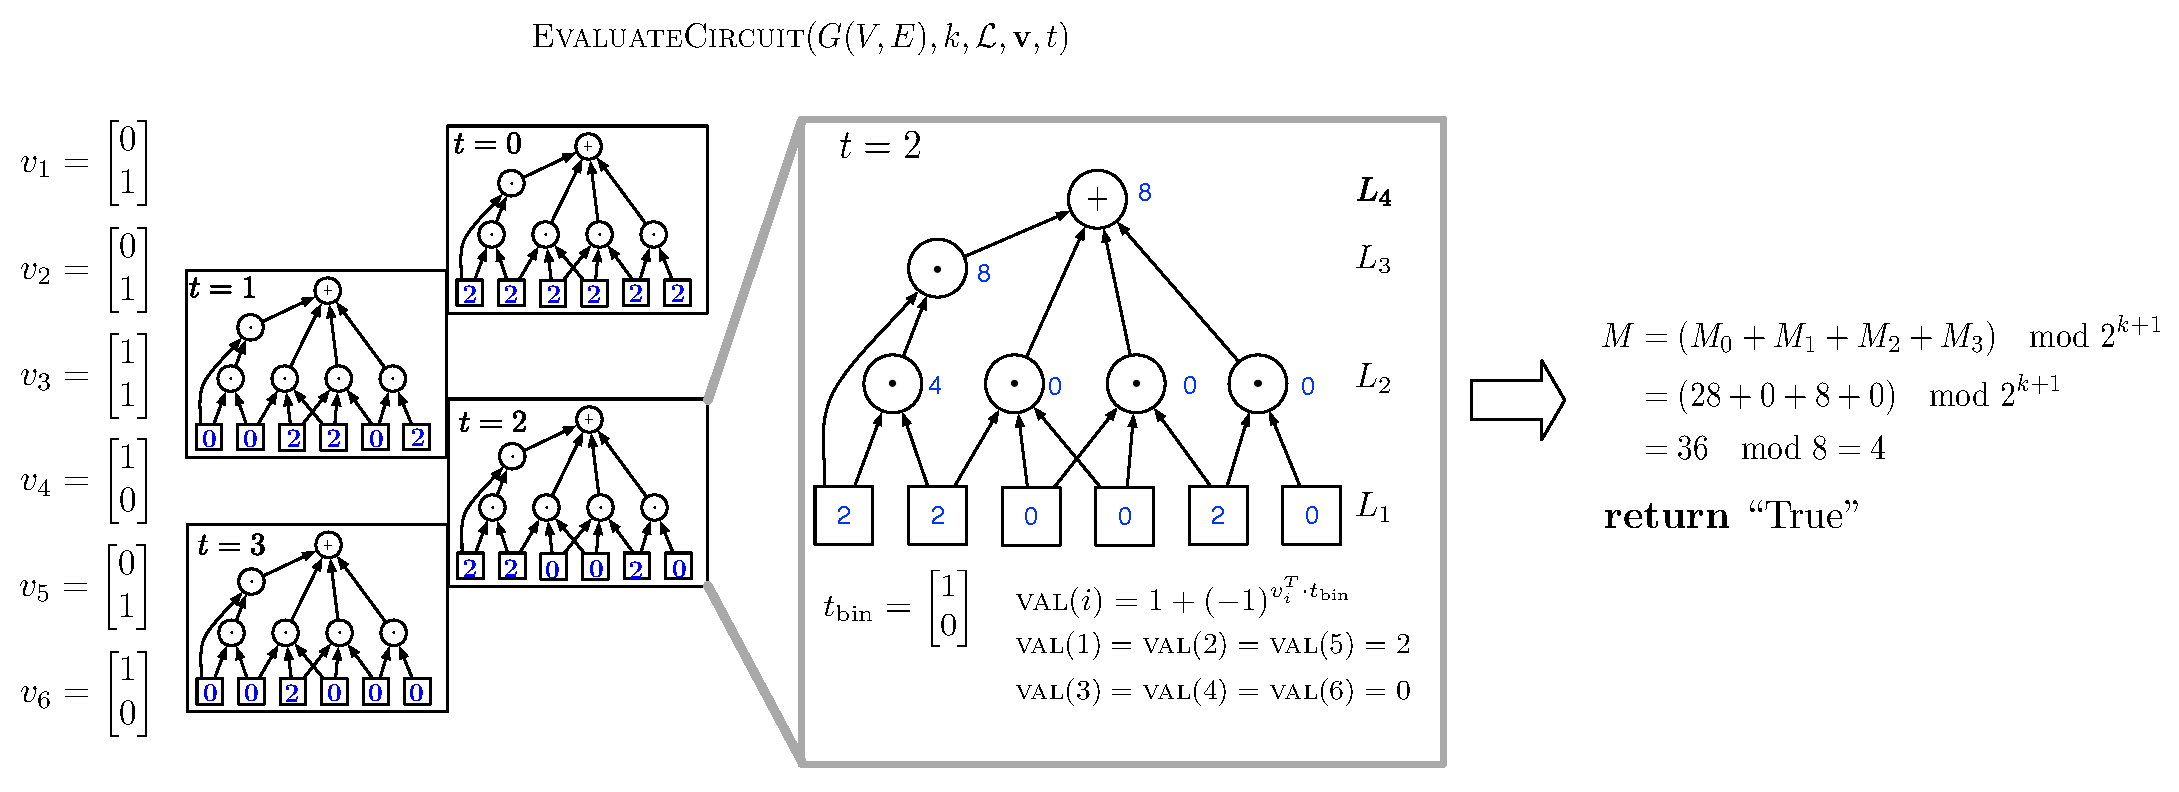
\includegraphics[width=\textwidth]{img/algorithm-example-v2_fixed.pdf}
\caption{
\small
Example of the sequential algorithm \maxwt{}. The input is the circuit $G(V,E)$ from
Figure \ref{fig:dag} with 12 nodes on four levels, $L_1$, $L_2$, $L_3$ and $L_4$, as shown.
The algorithm picks the vectors $v_1,\ldots,v_6$ from $\mathbb{Z}_2^2$, as shown in
the left of the figure. Since $k=2$, there are $2^k=4$ iterations, corresponding to
$t=0,\ldots,3$. The values of $\val(v)=1+(-1)^{v^Tt_{bin}}$ for the $t$th iteration
are shown in blue as the input values. The outputs of the circuit are $M_0, \ldots, M_3$,
with values as shown in the right of the figure. For these choices of the $v_i$'s, the
computed value $M\neq 0 (\text{mod } 2^{k+1})$, which implies the existence of a
multilinear term with $k$ variables. This is true because the term $x_5x_6$ in the
polynomial is indeed multilinear.
%---IDs are in red---$k=2$, and 3 levels. Nodes 1 through 6 are the first level---i.e., the circuit inputs. Nodes 7 through 10 are the second level, all with multiplication operation ($op(i) = \cdot$). The last level only contains the root of the circuit, with addition operation. First, the algorithm generates random vectors $v_i$ for the circuit inputs (bottom left). Then, the circuit is evaluated $2^k$ times by calling procedure \algcircuit{} (center). We show the evaluation for iteration $t=2$. First, we compute the inputs to the circuit as $1 + (-1)^{v_i^T\cdot t_{\text{bin}}}$---this will always be either 2 or 0. From there, we can evaluate the circuit by levels. Finally, back in \maxwt{}, we aggregate the value at root$(G)$ over all the iterations (right). In this case, the polynomial evaluates to $0$, so we return ``False".
%\vspace{-0.2in}
}
\label{fig:algorithm-example}
\end{figure*}

%\begin{algorithm}{}
%\small
%\caption{\maxwt{}$(G(V, E), k$.}
%\label{alg:multilinear-detect}
%\begin{algorithmic}[1]
%\STATE \textbf{Input}: Graph $G(V, E)$, parameter $k$
%\STATE\textbf{Output}: ``True" if circuit evaluation is non-zero. ``False" otherwise.
%\STATE \textbf{Initialize circuit inputs}
%\STATE \textbf{for} node $i \in L_1$ \textbf{do}
%\STATE \quad Let $v_i$ be a random vector from $\mathbb{Z}_{2}^k$
%\STATE \textbf{Initialize the polynomial}
%\STATE Let $M = \bar 0$
%\STATE \textbf{Evaluate circuit for each row of matrix representation}
%\STATE \textbf{for} $t = 0$ to $2^{k-1}$ \textbf{do}
%\STATE \quad $M_t = \algcircuit(G(V, E), k, \mathcal{L}, \mathbf{v}, t)$
%\STATE $M = \sum_{t=0}^{2^{k-1}} M_t \mod 2^{k+1}$
%\STATE \textbf{return} $M \neq 0$
%\STATE
%\STATE \textbf{procedure} \algcircuit{$(G(V, E), k, \mathcal{L}, \mathbf{v}, t)$}
%\STATE \textbf{Input}: Circuit $G(V, E)$, parameter $k$, node levels $\mathcal{L}$, random assigment $\mathbf{v}$, and iteration number $t$
%\STATE\textbf{Output}: Value at root node of $G(V,E)$
%\STATE \textbf{Initialize circuit inputs}
%\STATE \textbf{for} node $i \in L_1$ \textbf{do}
%\STATE \quad $ \val(i) = 1 + (-1)^{v_i^T \cdot t_{\text{bin}}}$
%
%\STATE \textbf{Evaluate the circuit by levels}
%\STATE \textbf{for} $s=2$ to $|\mathcal{L}|$ \textbf{do}
%\STATE \quad \textbf{for} $i \in L_s$ \textbf{do}
%\STATE \qquad \textbf{if} $\op(i) = +$ \textbf{then}
%\STATE \qquad \quad $\val(i) = 0$
%\STATE \qquad \quad \textbf{for} $j \in \pred(i)$ \textbf{do}
%\STATE \qquad \qquad $\val(i) = \val(i) + \val(j)$
%\STATE \qquad \textbf{else} 
%\STATE \qquad \quad $\val(i) = 1$
%\STATE \qquad \quad \textbf{for} $j \in \pred(i)$ \textbf{do}
%\STATE \qquad \qquad $\val(i) = \val(i) \cdot \val(j)$
%
%\STATE \textbf{return} $\val($root$(G))$
%\end{algorithmic}
%\end{algorithm}

\begin{algorithm}{}
\small
\caption{\small \textsc{MLD-ScanStat}$(G(V, E), \mathbf{w}, k, \epsilon, r)$.}
\label{alg:mld-scanstat}
\begin{algorithmic}[1]
\STATE \textbf{Input}: Instance $(G(V, E), \mathbf{w})$ and parameters $k, \epsilon, r$
\STATE\textbf{Output}: "True" if $G$ has a subgraph $S$ with size $i \leq k$ and weight $j \leq r$
\STATE Let $K=\{1,\ldots,k\}, R=\{0, \ldots, r\}$
\STATE \textbf{Initialize the polynomial}
\STATE $P(i, j) = \bar{0}$ for $i \in K$, $j \in R$
\STATE For each node $v$, pick a random vector $x_v \in Q[\mathbb{Z}_{2}^k]$
\STATE \textbf{Evaluate the circuit for each row of matrix representation}
\STATE \textbf{for} $t = 0$ to $2^{k-1}$
\STATE \quad $P_v(i, j) = \bar{0}$ for $i \in K$, $j \in R$
\STATE \quad \textbf{Initialize circuit inputs}
\STATE \quad \textbf{for} $v \in V$ \textbf{do}
\STATE \quad \quad $P_v(1, w(v)) = 1 + (-1)^{x_v^T \cdot t_{\text{bin}}}$
\STATE \quad \textbf{Evaluate circuit recursively}
\STATE \quad \textbf{for} $v \in V$, $i = 2$ to $k$, $j = 0$ to $r$ \textbf{do}
\STATE \qquad $P_v(i,j) = \sum_{u \in \nbr(v)} \sum_{i' = 1}^{i-1}\sum_{j'=0}^j (P_v(i', j') \cdot P_u(i-i', j - j'))$ 
\STATE
\STATE \textbf{return} $P \neq \bar 0$
\end{algorithmic}
\end{algorithm}

%\begin{theorem}[Koutis \cite{koutis:icalp08} and Williams \cite{williams2009finding}]
%\label{theorem:kmld2}
%Algorithm \maxwt{} correctly solves the \textsc{$k$-MLD} problem for an 
%instance $P(x_1,\ldots,x_n)$ with probability at least 1/5 in time
%$O(2^k poly(n))$ and space $O(2^k n)$.
%\end{theorem}

%We note that the success probability in Theorem \ref{theorem:kmld2} can be made very high,
%e.g., $1-\frac{1}{n}$, by running the algorithm $O(\log{n})$ times.
